%%%%% Inspection and Characterization Plan for DESC

%----------------------------------------------------------------------------------------
%	PACKAGES AND DOCUMENT CONFIGURATIONS
%----------------------------------------------------------------------------------------

\documentclass[12pt, a4paper]{article}

\usepackage{graphicx} % Required for the inclusion of images
\usepackage{natbib} % Required to change bibliography style to APA
\usepackage{amsmath} % Required for some math elements 

\setlength\parindent{0pt} % Removes all indentation from paragraphs

%\usepackage{times} % Uncomment to use the Times New Roman font

%----------------------------------------------------------------------------------------
%	DOCUMENT INFORMATION
%----------------------------------------------------------------------------------------

\title{Inspection and Characterization Plan} % Title

\author{Science Release and Validation team} % Author name

\date{\today} % Date for the report

\begin{document}

\maketitle % Insert the title, author and date

\begin{center}
Version 0.1
\end{center}

% If you wish to include an abstract, uncomment the lines below
% \begin{abstract}
% Abstract text
% \end{abstract}

%----------------------------------------------------------------------------------------
%	SECTION 1 -- the document's purpose is described, plus reference info
%----------------------------------------------------------------------------------------

\section{Purpose of the document}

This document is aimed at describing the process to execute the test suite necessary to characterize new Rubin data releases, in the context of the DESC. It covers the following points:

\begin{itemize}
\item Describe the purpose of having an additional layer of characterization tests, besides those coming from Rubin.
\item The list of tests, methods, tools and criteria (where applicable) to characterize and validate the Rubin dataset, for the purposes of DESC analyses.
\item The actual procedure for the execution of tests and inspection.
\end{itemize}

%\subsection{Changes from the last version}

\subsection{Definitions, reference documents}

\begin{itemize}
\item Test run: a single execution of the whole SRV characterization framework. Includes tests using DESCQA, other sources, inspection of data and documentation.
\item Test Execution Report (TER): a short document where the results of a Test run are summarized.
\end{itemize}
 
%----------------------------------------------------------------------------------------
%	SECTION 2 -- the purpose of the test runs is described
%----------------------------------------------------------------------------------------
\section{Goals of the characterization process}

The overall objective of the inspection and characterization procedure is to \textbf{provide a compiled snapshot of the characteristics of the data}, specifically for DESC scientists to refer to when using a specific Rubin or DESC science release for their analyses.

It is expected that the Rubin project will provide, alongside with the data itself, documentation and/or reports on the data quality, conducted by their own Verification and Validation tests. With the framework that SRV is providing here, the intention is to cater to the interests of the DESC ('fill the gaps'), in case some tests are missing from those provided by Rubin, evaluating the characteristics of 'typical' DESC science samples, testing DESC only value added products, and rechecking some basic metrics in case the data source is different than that of the Rubin Science Platform (e.g., if DESC uses a subset of the data in a different platform or format at NERSC).

A structured compilation of all the relevant tests and inspections will be finally recorded on static Test Execution Reports, which should contain all the information necessary for provenance and regression purposes.

At the same time, it is noteworthy to consider that the execution of these tests are easily run and re-run, and do not require a significant overhead in terms of execution and SRV (DESC) scientists' time, so as to make this framework useful as a quick assessment. A final overall evaluation of the data quality for a 'frozen' version of the data release can be done with a more comprehensive approach, as a final report usable as reference for downstream analyses. Therefore, any science done would be able to use the corresponding TER metrics and references, and minimize any ambiguities as to which version of the data or catalog content is used.

The overall characterization framework is sketched in Figure \ref{fig:srvplanning} and summarized below:

\begin{enumerate}
	\item Data is made visible for an official Release at the Science Platform. It is foreseen that part of this data is copied to NERSC. At this point, \textbf{inspection tests} through Jupyter notebooks can be performed quickly to assess overall data health. Examples: RA,DEC coverage; histograms of flags; other simple histograms of the main photometric quantities. It is interesting to verify whether the results are compatible at the Rubin Science Platform and at NERSC. These inspection \textit{could} be complemented by tests being run through other tools, if that seems to be more manageable (examples: running TOPCAT and acquiring data from the Rubin Science Platform through TAP, using Lite IDACs capabilities such as those from Hadoop frameworks holding a version of the data).
	\item At the same time, the presence of \textbf{adequate documentation} from Rubin side for DESC purposes, can be inspected, complementing it when appropriate or reporting back to the project.
	\item We should strive for the \textbf{main software tests to be run through a single framework (DESCQA)} as much as possible. These tests will be described in this document.
	\item It is possible however, that for practical purposes \textbf{some tests are not run through DESCQA} (already embedded in other frameworks, coming from downstream analyses). SRV has to analyze when that happens how and if to include them in the final report, ensuring consistency of the data sets used for the tests, with respect to those ran at DESCQA.
	\item Finally, besides the TER static reporting, SRV will explore the available dynamical \textbf{visualization utilities} for the test runs and re-runs that will inform the contents of the TER.
\end{enumerate}

\begin{figure}[h]
\begin{center}
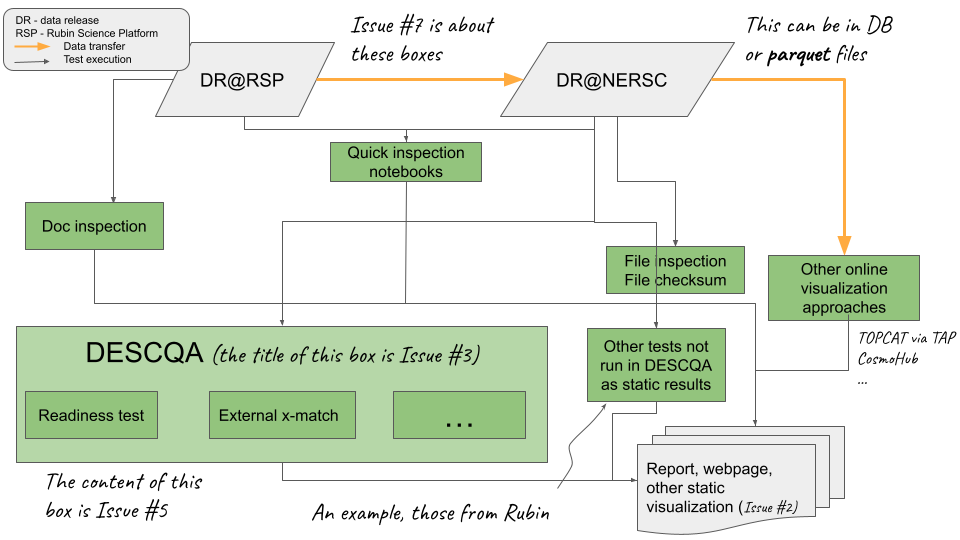
\includegraphics[width=0.95\textwidth]{../SRV_planning_diagram.png} 
\caption{SRV planning diagram}
\label{fig:srvplanning}
\end{center}
\end{figure}



%----------------------------------------------------------------------------------------
%	SECTION 3 -- the software and other tools are described
%----------------------------------------------------------------------------------------

\section{Test tool description}

Here we include an overall view of the software involved in a single test run of the SRV characterization framework.

\subsection{Software tools}

A list of references to the software used. The Test Execution Reports will be filled out with the actual versions and other specifics.

\subsection{Data sets and formats}

An explanation of the characteristics of the model of the data set being tested.

\subsubsection{DC2}

DC2 coadd catalogs is available as flat parquet files at NERSC.

\subsubsection{DP0.2}

TBC

%----------------------------------------------------------------------------------------
%	SECTION 4 -- the specific characterization cases and procedures are described
%----------------------------------------------------------------------------------------

\section{Characterization cases and procedures}

\subsection{Characterization of data set}

\subsubsection{TC1 - Inspection of catalog columns}
\textbf{Purpose:} 

Verify that the catalogs contain the columns we need.

\textbf{Strategy:} 

Execute an interactive job over the whole data set of the ColumnInspection test from DESCQA.

This can be a simple listing of all columns, and making an automatic check on whether certain columns exist or not. 
Another part can check for NaNs or crazy values in the relevant columns (similar to what the Readiness test does in DESCQA)

\textbf{Procedure:} 

Describe how we actually go about running this (./descqarun --t ColumnInspection --c DC2 etc.)

\subsubsection{TC2 - Basic recursive characterization}
\textbf{Purpose:} 

Run a general 'readiness' test on coadd catalogs, to verify that there aren't any significant issues in data. 

\textbf{Strategy:} 

Execute an interactive job over the whole data set of the CoreChecks test from DESCQA.

The test currently comprises the following checks:
\begin{itemize}
	\item RA,DEC scatter plot
	\item Differential magnitude histograms in all bands, for PSF, aperture and model magnitudes.
	\item Magnitude vs magnitude error scatter plots of the above.
	\item Color-color plots (specifics TBC)
	\item Magnitude vs size plots fpr PSF-like objects
	\item PSF ellipticity whisker plot
	\item Source e1,e2 histogram (TBC, requires some source selection)
\end{itemize}

\textbf{Procedure:} 

Describe how we actually go about running this (./descqarun --t CoreChecks --c DC2 etc.)
%\textbf{Regression:}

\subsubsection{TC3 - Notebooks}
Interactive notebooks to be included here that complement or substitute DESCQA executions, that could be run on NERSC and RSP. Also CosmoHub could be an option if the data is available.

\subsection{TC4 - Inspection of external tests on same data set}
Add details of other test runs on the same data set that will complement this report: RAIL, faro, other analysis WG results.

\subsection{Inspection of available documentation}
This requires reporting where the documentation of the data release is available.

\subsection{Validation tests on small areas or subsamples, replicating previous scientific results}

%----------------------------------------------------------------------------------------
%	SECTION 5 -- the reporting is described
%----------------------------------------------------------------------------------------

\section{Test execution reports and visualization}

The reports should include date, DESCQA version (and other SW), data set version, people involved in the testing. Then the results would be a summary of an online resource where the complete collection of plots and numbers would be available.


\end{document}